\documentclass[12pt]{article}
\usepackage{url}
\usepackage{graphicx}
\usepackage[hidelinks]{hyperref}
\usepackage{titlesec}
\usepackage{fancyvrb}
\usepackage{subcaption}
\usepackage{amsmath}

\newcommand{\innerproduct}[2]{\langle#1, #2 \rangle}
% \DeclareMathOperator*{\argmax}{arg\,max}
% \DeclareMathOperator*{\argmin}{arg\,min}
\usepackage{enumerate}
\usepackage{commath}
\usepackage{amssymb}
\usepackage[nottoc,numbib]{tocbibind}
\captionsetup{compatibility=false}
\graphicspath{ {./images/} }
\titleformat{\chapter}{}{}{0em}{\bf\LARGE}
\titlespacing*{\chapter}{0pt}{40pt}{10pt}

\usepackage{geometry}
 \geometry{
 a4paper,
 total={170mm,257mm},
 left=20mm,
 top=20mm,
 }

\usepackage{etoolbox}
\makeatletter
\patchcmd{\chapter}{\if@openright\cleardoublepage\else\clearpage\fi}{}{}{}
\makeatother

\title{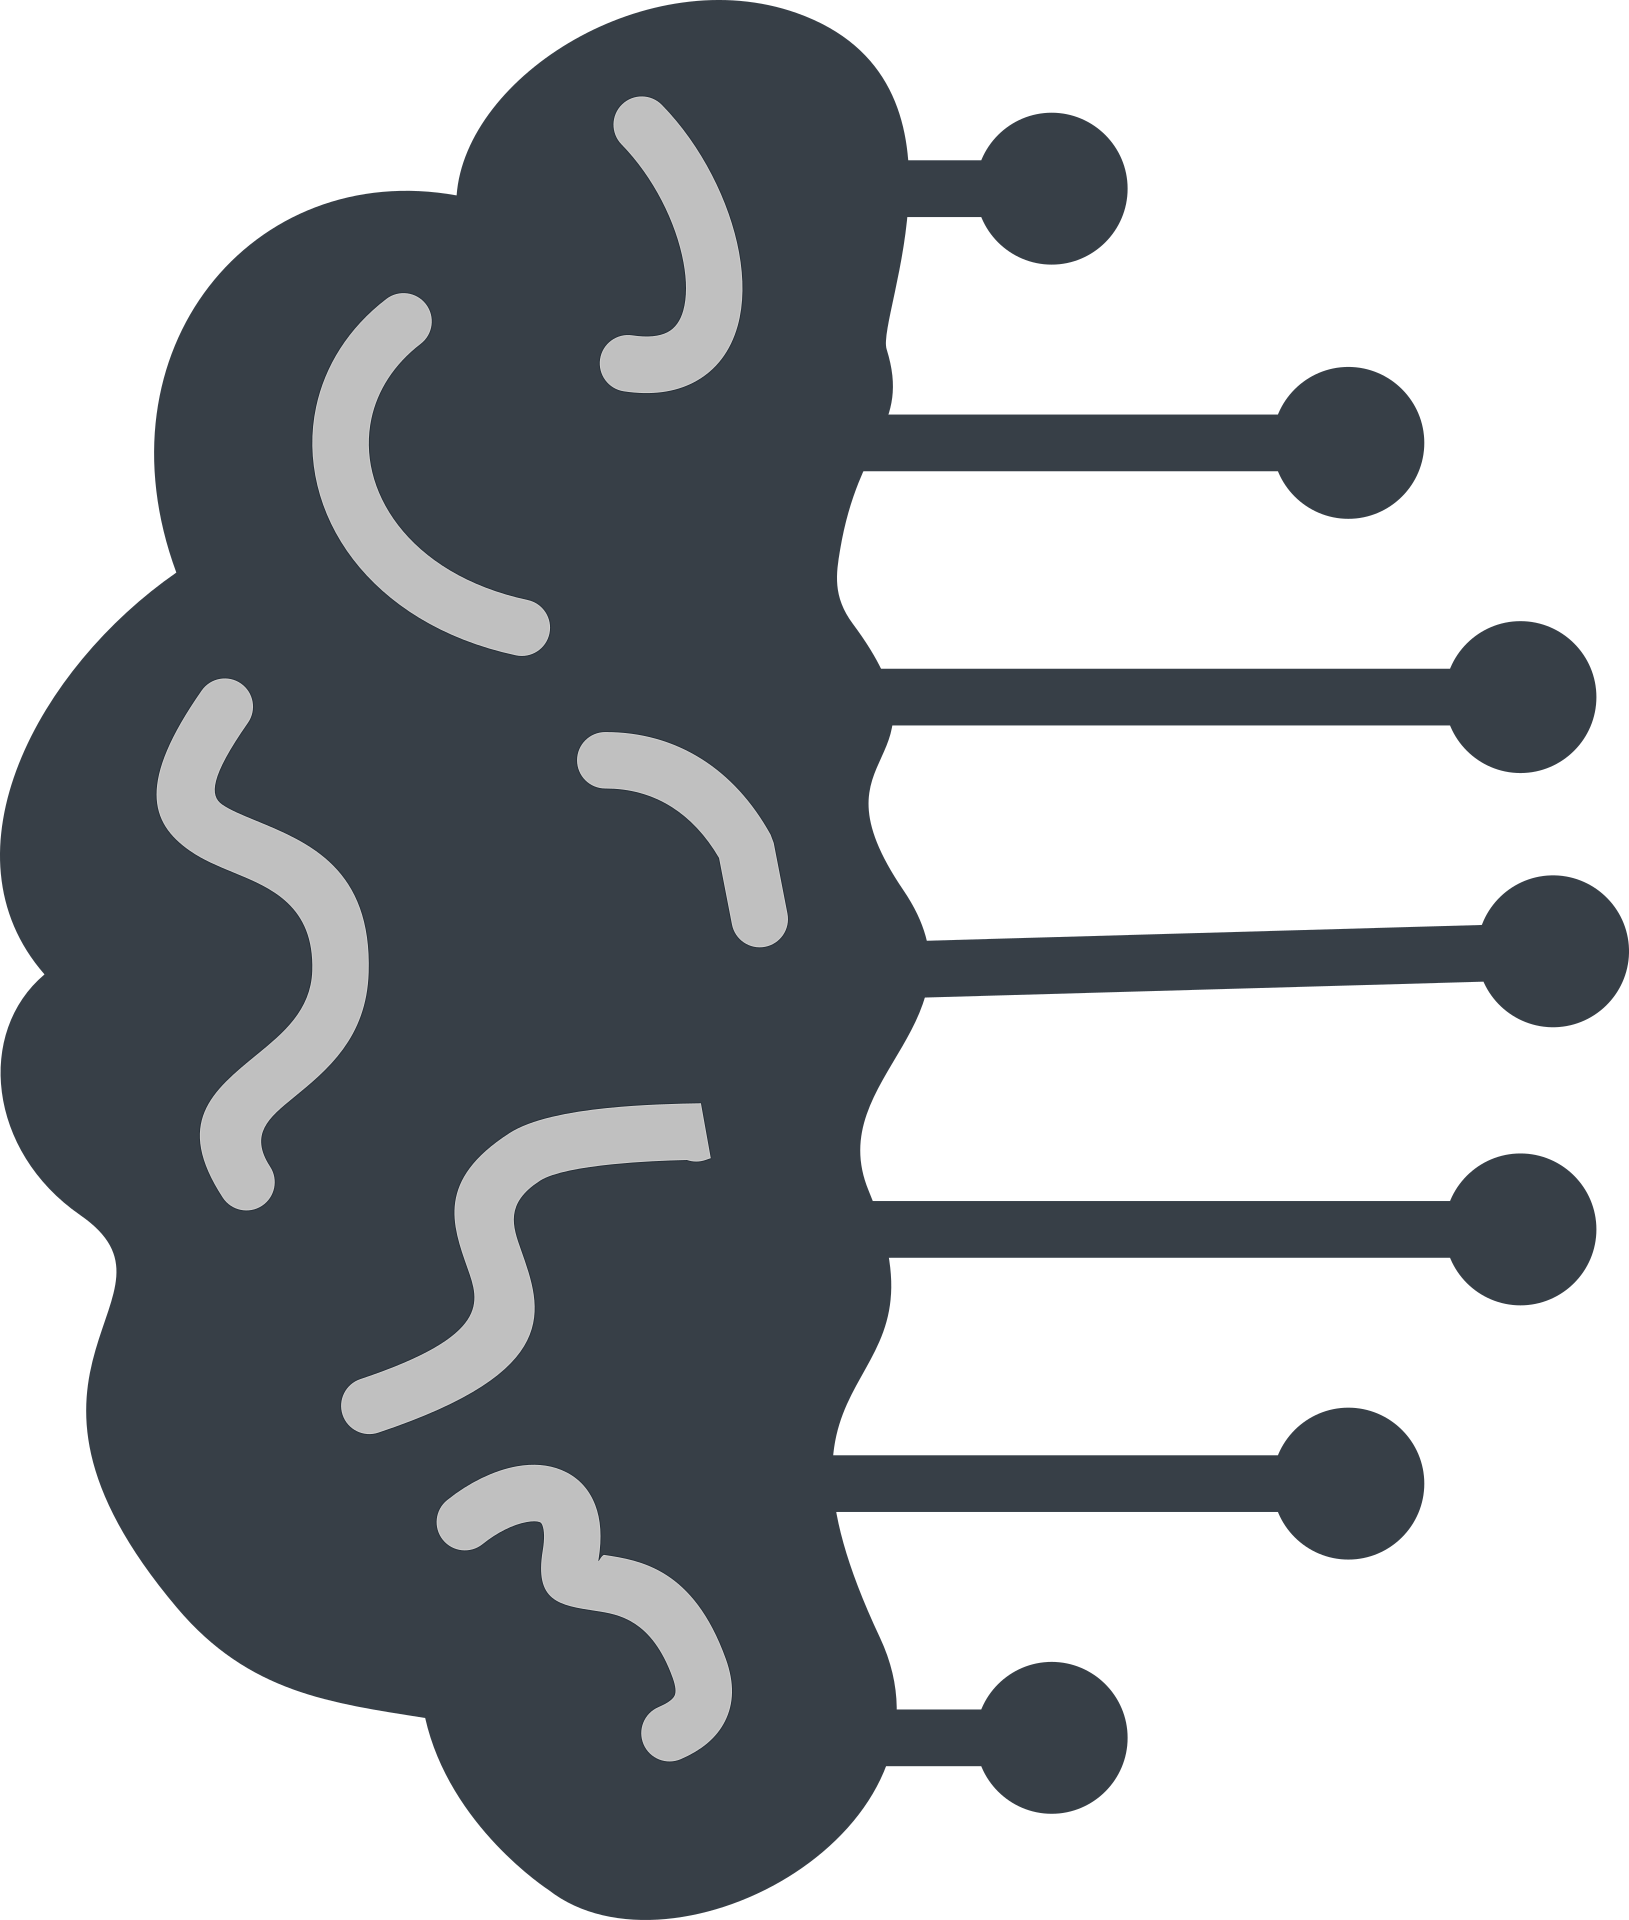
\includegraphics[width=8cm]{logo.png} \\[2cm] MIDTERM REPORT\\Machine Learning and Artificial Learning}
\author{Siddhant Mulkikar (23B0956)\\Mentor: Sabyasachi Samantaray}
\date{\today}

\begin{document}

\maketitle
\newpage
\tableofcontents
\newpage

\section{Objective}
This midterm report goes through the basics of Machine Learning, followed a dive into some popular ML algorithms.

\section{Introduction}
Machine Learning is the study of building mathematical models and algorithms to help understand data. It is often seen as a subset of artificial intelligence. Machine learning algorithms build a mathematical model based on sample data, known as "training data", in order to make predictions or decisions. 
\section{Categories in Machine Learning}
Machine learning can be broadly categorized into two main types: supervised learning and unsupervised learning.

\subsection{Supervised Learning}
Supervised learning involves training the model on a labelled dataset, which means that each training example is paired with the correct target value. The model aims to find a relationship or map from the input features to the labelled value, such that it can get the closely accurate target value for any prediction we ask from it.
It is further subdivided into two categories, regression and classification. Regression has continuous labels, like a real number in a range, while classification has discrete labels i.e. categories.
\subsection{Unsupervised Learning}
Unsupervised learning involves modelling the underlying structure or distribution in the data in order to learn more about the data. The model is trained on an unlabelled dataset, which means that the model is not provided with the correct target value.
These models involve algorithms like clustering, anomaly detection and dimensionality reduction. Clustering involves grouping similar data points together, while dimensionality reduction involves reducing the number of input variables in the dataset, representating the data more clearly and anomaly reduction involves detecting outliers in the data.

\section{Model Selection}
\subsection{Hyperparameters}
A hyperparameter is a parameter, such as the learning rate or batch size, which specifies details of the learning process. These are set before the learning process and are not interfered with while fitting the model to the training set. Hyperparamters usually tend to decide the efficiency of the model, and therefore, need to be tuned and optimized to get the most accurate predictions from the model.

\subsection{Model validation}
Model validation is important to check the effectiveness of our model, and this is done after choosing the model and the hyperparameters associated with it. However the limitaion we have is that our training set is limited, which forces us to develop ways to validate based on the limited data we have.
\subsubsection*{Holdout sets}
In this method, a subset of data is withheld from the training set, and then this data is used to check the model performance by predicted the target variables for this holdout set and comparing it with its labels. The problem with this is we are reducing the already limited size of training examples even more. This is where cross validation comes in.
\subsubsection*{Cross Validation}
In cross validation, the training set is divided into subsets of equal size, and the model is trained on all of them individually, while the remaining set is used to validate the model. This is repeated for all the subsets and the final validation score is gotten by combining all the validation scores from each subset, which can be done by taking the mean or some other way. This method is more effective than holdout sets, because none of the training examples are lost in the process.
\begin{center}
    \includegraphics*[width=15cm]{cv.png}\\
    Five-fold cross validation
\end{center}
\newpage 


\section{Supervised Learning Algorithms}
\subsection{Linear Regression}
Linear regression is a good starting point for regression models. The simplest linear regression model is fitting a straight line to a dataset, but it can be extended to model more complicated data behaviour.
% \textbf{Simple Linear Regression: }\\
% A straight line fit is a model of the form : 
The simplest linear regression model is a straight line fit, which is a model of the form :
\begin{equation}
    f_{w,b}(x) = \innerproduct{w}{x} + b
\end{equation}
The ultimate goal of the model is to find a weight vector $w$ and bias $b$, such that the predicted value of the target variable is as close as possible to the actual value over all training examples.
\\Given a input feature vector $x = <x_1,x_2,\dots,x_m>$, the model predicts the output $\hat{y}$, which is called the target variable, as:
\begin{equation}
    \hat{y} = f_{w,b}(x) = \innerproduct{w}{x} + b
\end{equation}
where, $w = <w_1,w_2,\dots,w_m>$ is a vector of weights, $b$ is the bias term, both of which are learned by the model during the learning process.
\begin{center}
    \includegraphics*[width=10cm]{lin-reg.png}\\
    Straight line fit after linear regression
\end{center}
In order to train the model, a cost function is defined, which measures the accuracy of the model's prediction. One of the most popular cost functions for linear regression is Mean sqaured error (MSE), which measures the average sqaure deviation between the actual and predicted target, values which is defined as:
\begin{equation}
    MSE = \frac{1}{m} \sum_{i=1}^{n} (y^i - \hat{y^i})^2 = L(w,b)
\end{equation}

The model is trained by updating the weight vector $w$ such that the cost function is minimized, which is done by using another algorithm like gradient descent. 

\subsubsection*{Gradient Descent}
Gradient descent is an optimization algorithm used to minimize some function by iteratively moving in the direction of steepest descent as defined by the negative of the gradient. The algorithm updates the weights vector and bias on each iteration, till it reaches a minima for the cost function.
\begin{equation}
    w' = w - \alpha \frac{\partial L(w,b)}{\partial w}
\end{equation}
\begin{equation}
    b' = b - \alpha \frac{\partial L(w,b)}{\partial b}
\end{equation}
where $\alpha$ is the learning rate, which determines the size of the step taken in the direction of the gradient, and can be tuned to get the best predictions. 
If the number of training examples are $m$ and the number of features are $n$, then the gradient of the cost function with respect to the bias and $j^{th} weight$ is given by:
\begin{equation}
    \frac{\partial L(w,b)}{\partial b} = \frac{2}{m} \sum_{i=1}^{m} (\hat{y^i}-y^i)
\end{equation}
\begin{equation}
    \frac{\partial L(w_j,b)}{\partial w_j} = \frac{2}{m} \sum_{i=1}^{m} {x_j}^i(\hat{y^i}-y^i)
\end{equation}
\begin{center}
    \includegraphics*[width=\textwidth]{grad-descent.png}
\end{center}
However, gradient descent can give inaccurate predictions if the algorithm doesn't reach the minima, i.e. it diverges from the minima. The convergence of gradient descent into a minima is determined by the learning rate $\alpha$.

\subsubsection*{Learning rate $(\alpha)$}
Learning rate is a hyperparameter that determines the size of the step taken in each iteration of gradient descent. 
% insert image of learning rate
\begin{center}
    \includegraphics*[width=\textwidth]{lr-types.png}
    $L(w)$ vs $w$ for different learning rates $\alpha$
\end{center}
Lets go through all the cases to see how the learning rate affects the convergence of the gradient descent:
\begin{itemize}
    \item \textbf{Small learning rate:} If $\alpha$ is too low, the algorithm might take a lot of time to converge to the minimum, as the size of step is too small.
    \item \textbf{Optimal learning rate:} If $\alpha$ is chosen properly, gradient descent converges to the minima in a decent number of epochs, which is desired.
    \item \textbf{Large learning rate:} If $\alpha$ is high, it takes a big step during each iteration, such that it might overstep the minima and end up on the other side of the minima. This might result in a delayed convergence or no convergence at all.
    \item \textbf{Too High learning rate:} If $\alpha$ is too high, the cost function would diverg, which might end up increasing the cost function, instead of minimizing it in each iteration.
\end{itemize}

\subsection{Polynomial Regression}
Conceptually, polynomial regression is pretty similar to linear regression. The difference is instead of fitting a straight line, a polynomial curve is fitted to the data.\\
Lets consider an univariate polynomial regression model ($n=1$), for simplicity, of degree $d$, with the weights being $w=<w_1,w_2,\dots,w_d>$. The model is this case would be:
\begin{equation}
    f_{w,b}(x) = w_1x + w_2x^2 + \dots + w_dx^d + b
\end{equation}

This can be thought of a linear regression model of $d$ features, where the features are not independent. Thus, the input feature vector would be $\vec{x}=<x,x^2,\dots,x^d>$ and the model would be $f_{w,b}(x) = \innerproduct{w}{\vec{x}} + b$.\\
\begin{center}
    \includegraphics*[width=10cm]{poly-reg.png}\\
    Polynomial curve fit after polynomial regression
\end{center}

\subsection{Logistic Regression}
Despite the name suggesting regression, logistic regression is usually used as a binary classification model, i.e. it has two target variable values - 1 and 0, or True and False, also known as classes. 
Given an input feature vector $x = <x_1,x_2,\dots,x_m>$, the model gives the probability of the target variable being 1, as:
\begin{equation}
    f_{w,b}(x) = \sigma(\innerproduct{w}{x} + b) = P(\hat{y}=1|x)
\end{equation}
where $\sigma$ is the sigmoid function, defined as:
\begin{equation}
    \sigma(z) = \frac{1}{1+e^{-z}}
\end{equation}
The sigmoid function maps any real number to the range (0,1), which is useful for binary classification, as it can be interpreted as the probability of the target variable being 1.\\
\newline
If the input vectors and their labels are represented as points in the vector space, the hyperplane $z = w \cdot x + b$, divides the vector space into two regions, i.e. two classes, henceforth classifying the dataset.
\newline
While one might think of using the MSE cost function for logistic regression, it turns out that the loss function is not convex, which means that gradient descent might not converge to the minima. Hence a different cost function known as the logistic loss function is used, which is defined as:
\begin{equation}
    L(f_{w,b}(x),y) = \frac{1}{m} \sum(-y \log(f_{w,b}(x)) - (1-y) \log(1-f_{w,b}(x)))
\end{equation}

Gradient descent can used here to train the model in the similar way as linear regression.
The gradients for the $j^{th}$ weight and the bias are given by:
\begin{equation}
    \frac{\partial L(w,b)}{\partial b} = \frac{1}{m} \sum_{i=1}^{m} (f_{w,b}(x)-y^i)
\end{equation}
\begin{equation}
    \frac{\partial L(w_j,b)}{\partial w_j} = \frac{1}{m} \sum_{i=1}^{m} x_j(f_{w,b}(x)-y^i)
\end{equation}


\subsection{Naive Bayes}
Naive Bayes models are a set of supervised learning algorithms based on the Bayes theorem, which is:
\begin{equation}
    P(A|B) = \frac{P(B|A)P(A)}{P(B)}
\end{equation}
Lets consider a dataset with $n$ discrete features at first. The probability of the desired class $y$ for a single input feature $x_i$, is given by:
\begin{equation}
    P(y|x_i) = \frac{P(x_i|y)P(y)}{P(x_i)}
\end{equation}
Considering the dataset has $n$ features, the model calculates the probability of the desired class $y$ for the input feature vector $x = <x_1,x_2,\dots,x_n>$, as:
\begin{equation*}
    P(y|x_1,x_2,\dots,x_n) = \frac{P(x_1,x_2,\dots,x_n|y)P(y)}{P(x_1,x_2,\dots,x_n)}
\end{equation*}
\begin{equation*}
    P(y|x_1,x_2,\dots,x_n) = \frac{P(y|x_1)P(y|x_2)\dots P(y|x_n)P(y)}{P(x_1)P(x_2)\dots P(x_n)}
\end{equation*}
\begin{equation}
    P(y|x_1,x_2,\dots,x_n) \propto P(y) \prod_{i=1}^{n} P(x_i|y)
\end{equation}

If the problem is of binary classifcation, with the classes being $y_1$ and $y_2$, we can decide between the two classes by taking the ratio of both the probabilities i.e. $\frac{P(y_1|x_1,x_2,\dots,x_n)}{P(y_2|x_1,x_2,\dots,x_n)}$ and check if this ratio is greater or lesser than 1.\\
More generally for multi-class classification, the class with the highest probability $\hat{y}$ is chosen as the predicted class by: 
\begin{equation}
    \hat{y} = \arg \max_{y} P(y) \prod_{i=1}^{n} P(x_i|y)
\end{equation}
\subsubsection*{Gaussian Naive Bayes}
If instead of discrete features, our model has continuous features, the Gaussian Naive Bayes model can be used. The only difference is the way in which the probabilities are calculated. While it is quite self-evident in the case of discrete features, it is not that obvious in the case of continuous features.\\
The model assumes that the dataset has a Gaussian distribution for each of the classes with no covariance between features (dimensions) i.e. every feature is independent from the other and then calculates the standard deviation $\sigma_y$ and $\mu_y$ for the desired class $y$, after which the probability for each feature is calculated as:
\begin{equation}
    P(x_i|y) = \frac{1}{\sqrt{2\pi\sigma_y^2}} exp \left (-\frac{(x_i-\mu_y)^2}{2\sigma_y^2}\right)
\end{equation}
% insert gaussian image
The steps after this are the same as in the discrete features case.
\begin{figure}[h]
    \begin{subfigure}{0.5\textwidth}
    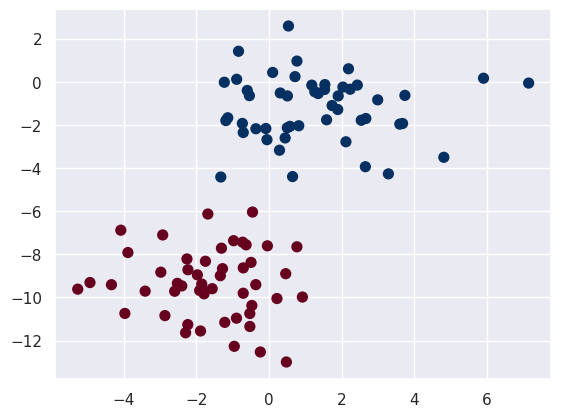
\includegraphics[width=\linewidth]{gaus-nb-before.png} 
    \caption{Representation of data points}
    \label{fig:subim1}
    \end{subfigure}
    \begin{subfigure}{0.5\textwidth}
    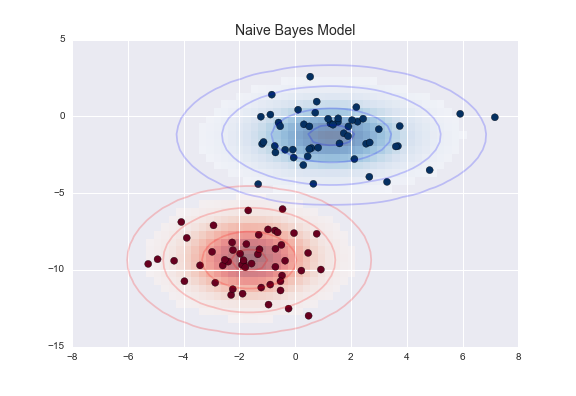
\includegraphics[width=\linewidth]{gaus-nb-after-2.png}
    \caption{After Gaussian Naive Bayes}
    \label{fig:subim2}
    \end{subfigure}
\end{figure}
\newpage
\subsection{Support Vector Machines}
A support vector machine is an supervised learning algorithm usually used for classfication problems. The model is similar to logistic regression, in the sense, that it fits a hyperplane, also known as decision boundary, separating the classes in two or higher dimensions. However, the difference lies in choosing the hyperplane.\\
Lets consider a binary classification problem, with two classes $y_1$ and $y_2$. As we can see in the figure below, there are multiple hyperplanes which can be separators, and the choice of a hyperplane would affect the class which would be assigned to a new input data point, i.e. the red cross in the plot.\\
\begin{center}
    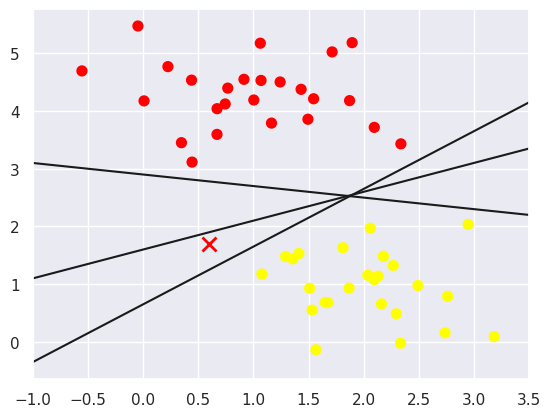
\includegraphics[width=10cm]{svm-possible-hp.png}
\end{center}
SVMs solve this problem by fixing the choice of the hyperplanes. This is done by using a line of non-zero width as the hyperplane, instead of a zero-width line.\\
The original hyperplane is called the \textbf{maximum margin hyperplane}, which we will refer to as MMH hereafter for convenience.
The data points which are the closest to the MMH are called the \textbf{support vectors}. Two parallel hyperplanes to the MMH which pass through these support vectors are called \textbf{marginal planes}. The width between the marginal planes is called the \textbf{margin}.\\
SVMs aim to maximise this margin to get the optimal hyperplane for separation.
\begin{center}
    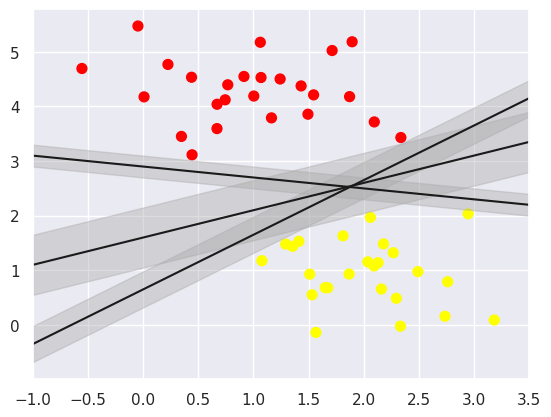
\includegraphics[width=10cm]{svm-margin.png}
\end{center}
Let a hyperplane be defined as:
\begin{equation*}
    \innerproduct{w}{x} + b = 0
\end{equation*}
Let the classes be linearly seperable, i.e. they can be separated by a single line between them. If $y_i = 1$, let the point belong to $y_1$, and if $y_i = -1$, let the point belong to $y_2$. Taking  the margin $2M$, we get 
For the hyperplane to be the MMH, the following conditions must be satisfied for all $i=1,2 \dots n$, where $n$ is the number of training examples, i.e. the number of data points:
\begin{enumerate}[(I)]
    \item $y_i(\innerproduct{w}{x_i} + b) \geq 1$ 
    \item $\max_{w,b} M$
\end{enumerate}
Let's choose a scale for the axes of the data such that $\innerproduct{w}{x} +b = 1$ at the closest data point $x_a$ to the hyperplane. Let the orthogonal projection of $x_a$ on the hyperplane be $x_a$'. By definition, it should satisfy the eqaution of the hyperplane.
\begin{equation}
    \innerproduct{w}{x_a'} + b = 0
\end{equation}
$\because$ $x_a = x_a' + M\frac{w}{\norm{w}}$, as $\frac{w}{\norm{w}}$ is the unit vector in the direction of $w$. Substituting this in (19), we get:
\begin{equation*}
    w \cdot (x_a - M\frac{w}{\norm{w}}) + b = 0
\end{equation*}
\begin{equation*}
    (w \cdot x_a + b) - M\norm{w} = 0
\end{equation*}
Since, $w \cdot x_a + b = 1$, we get:
\begin{equation}
    M = \frac{1}{\norm{w}}
\end{equation}

Hence, the second condition can be written as:
\begin{equation}
    \min_{w,b} \norm{w}
\end{equation}
In case of hard margin SVM classifiers, no misclassifcations can be allowed, i.e. the first condition must be satisfied for all $i=1,2 \dots n$. For this classifer, the cost function can be defined as:
\begin{equation}
    L(w,b) = \frac{1}{2} \min_{w,b} \norm{w}^2
\end{equation}

However, there can be overlaps between classes, for which soft margin SVM classifiers are used, which also allowed for misclassifcations and integrates this into the cost function.
The model defines a slack variable $\zeta_i$ for $i_{th}$ point, where $\zeta_i = \max(0,1-y_i(w \cdot x_i + b))$. 
The cost function therefore can be defined as:
\begin{equation}
    L(w,b) = \frac{1}{2} \min_{w,b} \norm{w}^2 + C \sum_{i=1}^{n} \zeta_i
\end{equation}
The value of $C$ is a hyperparameter, which decides the hardness of the margin. A large $C$ means a hard margin, i.e. it does not allow for points to lie in the margin, while a model with a small $C$ does allow for encompassing points.\\
In the case of non-linearly seperable data, kernels are used which project the data to a higher-dimensional space defined by the kernel function.
\begin{center}
    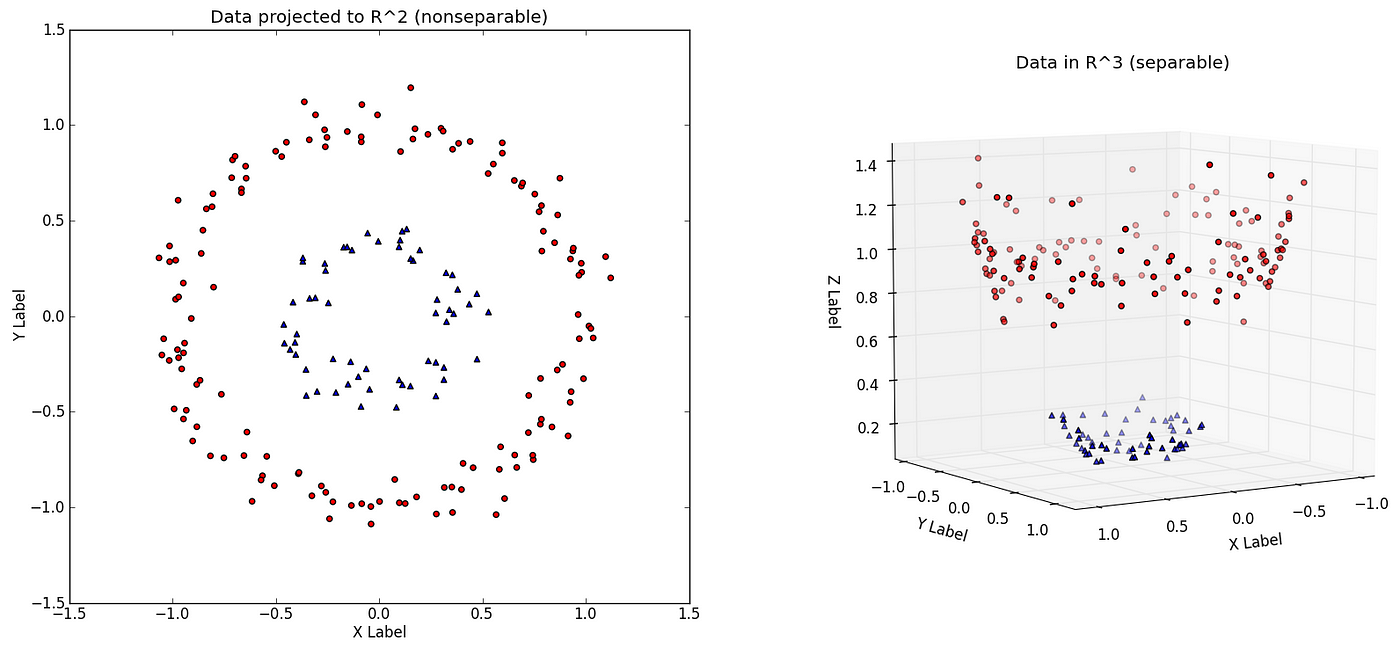
\includegraphics[width=\textwidth]{kernel.png}
\end{center}
Taking an example of a non-linearly separable dataset in $R^2$  in the above figure, the data can be projected to $R^3$ by using the radial basis function (RBF) kernel, which is defined as:
\begin{equation}
    K(x,x') = exp(-\gamma \norm{x-x'}^2)
\end{equation}
Now, a hyperplane can be easily constructed in $R^3$, separating the datasets in two classes. This results in an almost circular (non-linear) decision boundary in $R^2$.
\subsection{Decision Trees}
Decision trees is a non-parametric supervised learning algorithm used for classifcation and regression tasks. The model is structured as a rooted tree, consisting of nodes, which are essentially conditions. Each parent node splits into child nodes based on the condition in the node. The tree ends with the leaf nodes, i.e. the stage where the classification or regression is deemed to be completed.\\

\begin{center}
    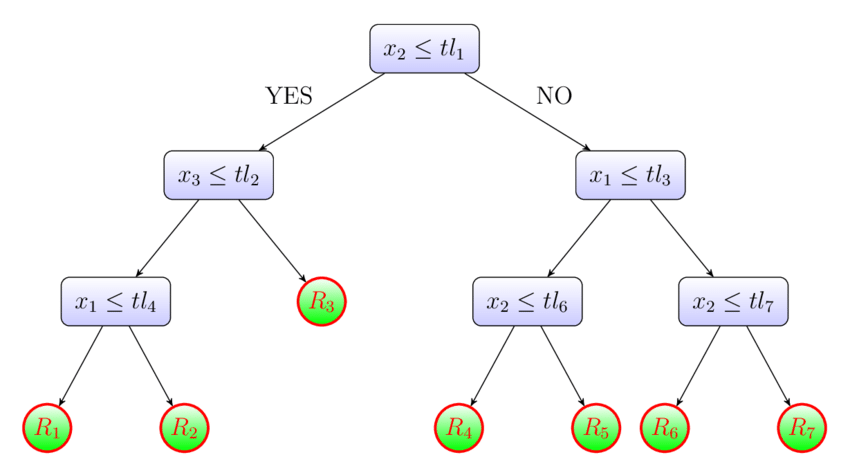
\includegraphics[width=10cm]{decision-tree-eg.png}
\end{center}
Lets consider we have some points in n-dimensions, marked red and blue. Taking a binary decision tree for this classification task, we start with the root node and compare the value of $x_2$ with the threshold value $tl_1$. Based on this condition, the whole n-dimensional space, splits into two regions, and with it the points are also seperated. This process is repeated for each node, where the region passed down from its parent node is splitted further based on the condition of the current node, till the leaf nodes are reached. \\
Considering the above example, there are 7 leaf nodes, each indicates a non-overlapping region in the n-dimensional space. Splitting at each node can be thought of putting a hyperplane in the n-dimensional space, basically a mini-decision boundary.\\
The optimal decision tree divides the n-dimensional space into regions, such that each region has only one class of points, which depends on the condition on the nodes. While, the model is said to be non-parametric, the conditions can be thought of parameters, which the model has to learn. This is done by maximising the \textbf{information gain} at each split, which is defined as:\\
\begin{equation}
    IG = E(parent) - \sum{E(child_i)}
\end{equation}
where $IG$ is the information gain, $E(Data)$ is the entropy of the data before the split and $E(Data|Split)$ is the entropy of the data after the split. The entropy of the data is defined as:
\begin{equation*}
    E(Data) = -\sum_{i=1}^{n} p_i \log_2(p_i)
\end{equation*}
where $p_i = n_i/n$ such that $n_i$ is the number of points of the $i_{th}$ class in the region of the node.\\
From this we can see that decision trees are greedy algorithms as the prioritise the decision which gives the most reward at the current node, without considering any future nodes.\\
\newline
Decision trees can be prone to overfitting and can take a lot of time to train, if not stopped from growning. This can be controlled by setting a maximum depth for the tree, or a minimum number of samples required to split a node, which are essentially hyperparameters set by the user.\\
\subsection{Random Forests}
Random forests, simply put, can be thought of as a collection of decision trees, which are trained parallely and then the final prediction is made by merging the outputs of all the individual trees. Hence, it is an ensemble learning method, which means utilising multiple learning algorithms to obtain the prediction.\\
Ensemble primarily can be of two types, Bagging and Boosting. Bagging is when the models are trained parallely, while Boosting is when the models are trained sequentially, with the output of one model being the input of the next model. \\
Random forests work on the principle of Bagging.
\subsubsection*{Bagging}
Bagging stands for Bootstrap Aggregation. The steps involved in bagging are:
\begin{enumerate}
    \item \textbf{Bootstrap: }Random subsets of training data is selected with replacement, allowing for multiple instances of the same data point. Each of these subsets is to be trained on a differene decision tree. 
    \item \textbf{Feature selection: }For each sample, a random subset of features is selected, such that the decision tree can split based on only these selected features. The size of this random subset is a hyperparameter, which can be tuned. However, the general consensus by researchers is that the log or square root of the total number of features works best.
    \item \textbf{Training: }A decision tree is trained on each of the bootstrap samples, with the selected features. 
    \item \textbf{Aggregation: }To get the final prediction, the input data point is passed through all decision trees, and the majority output is assigned as the class of the input data point, in the case of a classification problem. For regression, usually, the average of all the outputs is taken.
\end{enumerate}
Random forests, while slower, usually perform better than singular decision trees, as they are more robust and thus less prone to overfitting. Decision trees have a high variance and can change a lot with minor changes to the training data, whereas random forests are more resistant to such changes. They also help in feature selection by highlighting important features. 

\section{Deep Learning}
Deep learning is a subset of machine learning, which is based on neural networks. But before we get into deep learning, lets understand what a neural network is and how it works.
\subsection{Neural Networks}
Neural networks is a machine learning model, closelt inspired by the actual human brain and nervous system. It consists of many nodes, called neurons, arranged sequentially. Each layer is connected to the next layer. The first layer is called the input layer and the last layer is called the output layer. The layers in between are called hidden layers.\\
\begin{center}
    
\includegraphics[width=10cm]{nn-first.png}
\end{center}
As evident from the name, the input layer takes the input data, which is then passed through all the hidden layers, finally ending at the output layer, which gives the prediction. Each neuron takes an input and applies a function or mutltiple functions before passing the transformed input to the next layer.\\
\subsubsection*{Neuron}
A neuron is the basic unit of a neuron network. It takes a input vector $x = <x_1,x_2,\dots,x_n>$ from the previous layer. Each neuron has a weight vector $w = <w_1,w_2,\dots,w_n>$ and bias $b$ associated with it. The neuron first applies a linear function on the input:
\begin{equation*}
    z = \innerproduct{w^T}{x} + b
\end{equation*}
Then, an activation function $a$ is applied on z:
\begin{equation}
    a(z) = g(z)
\end{equation}
\newpage
Now lets consider the $L^{th}$ layer. For any term Q, let $Q^{[L]}$ denote the term in the $L^{th}$ layer. Hence, the number of neurons in this layer be $n^{[L]}$. The weight vector for the $j^{th}$ neuron would be $w^{[L]}_j$ and the weight matrix for the entire layer would be $w^{[L]}$ and the bias matrix to be $b^{[L]}$. Let the input to this layer be $X^{[L]}$.
\begin{equation}
    z^{[L]} = w^{[L]}X^{[L]} + b^{[L]}
\end{equation}
\begin{equation}
    z^{[L]} = \begin{bmatrix} w^{[L]}_1 \\ w^{[L]}_2 \\ \vdots \\ w^{[L]}_{n^{[L]}} \end{bmatrix} \begin{bmatrix} x_1 \\ x_2 \\ \vdots \\ x_n \end{bmatrix} + \begin{bmatrix} b^{[L]}_1 \\ b^{[L]}_2 \\ \vdots \\ b^{[L]}_{n^{[L]}} \end{bmatrix} = \begin{bmatrix} \innerproduct{w^{[L]}_1}{x} + b^{[L]}_1 \\ \innerproduct{w^{[L]}_2}{x} + b^{[L]}_2 \\ \vdots \\ \innerproduct{w^{[L]}_{n^{[L]}}}{x} + b^{[L]}_{n^{[L]}} \end{bmatrix}
\end{equation}
\begin{equation}
    a^{[L]} = g(z^{[L]})
\end{equation}
Since, for a hidden layer, the input is the output of the previous layer, i.e. $a^{[L-1]}=X^{[L]}$, and the input layer can be written as $a^{[0]}$. The equation can hence be written as:
\begin{equation}
    a^{[L]} = g(w^{[L]}a^{[L-1]} + b^{[L]})
\end{equation}

\subsubsection*{Activation function}
An activation function plays an important role in a neural network by introducing non-linearity in it. Without it, the entire network would be linear and can be representated by a single layer, simplifying the NN to a linear regression model, which we don't want as complexity is desired for better predictions.\\
There are many choices of activation functions available. Some of the popular ones are:
\begin{itemize}
    \item \textbf{Sigmoid: }$g(z) = \frac{1}{1+e^{-z}}=a$ and $a' = a(1-a)$\\
        \begin{center}
            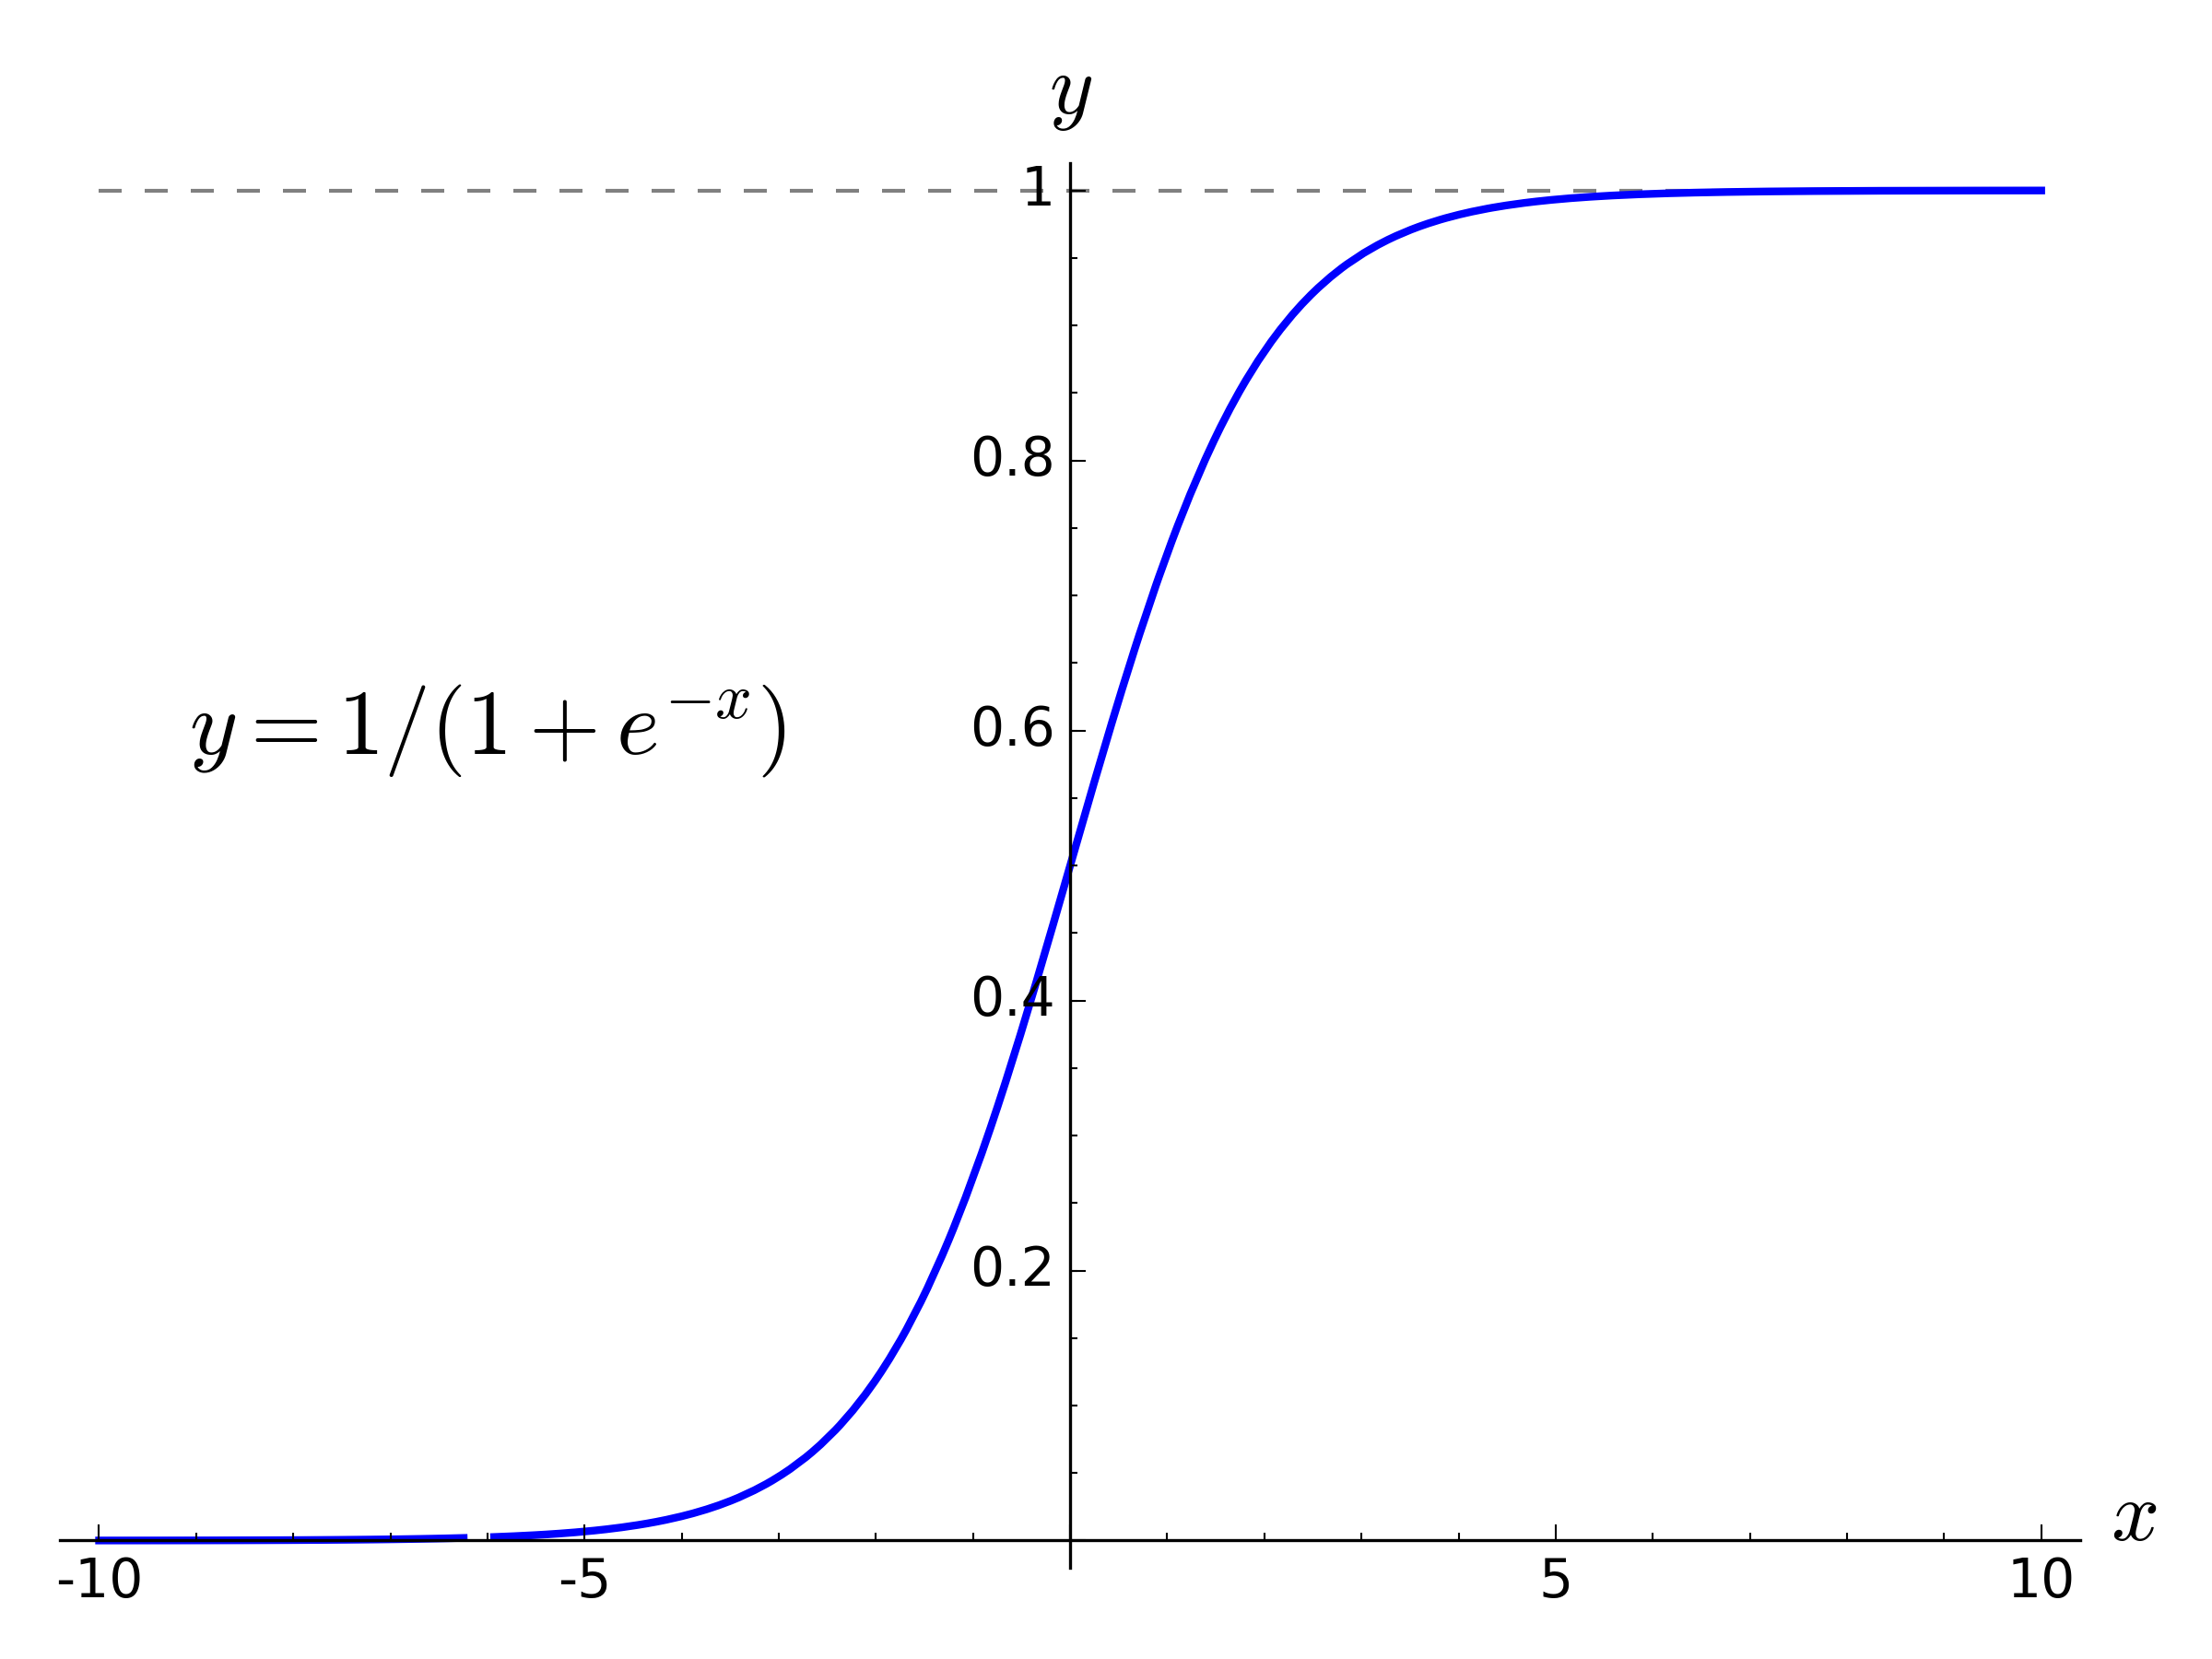
\includegraphics[width=6cm]{sigmoid.png}
        \end{center}
    \item \textbf{Tanh: }$g(z) = \frac{e^z - e^{-z}}{e^z + e^{-z}}=a$ and $a' = 1-a^2$\\It is a shifted sigmoid function, used to mean the data to 0. Usually it is prefered to sigmoid, except the last layer, where sigmoid is used.
        \begin{center}
            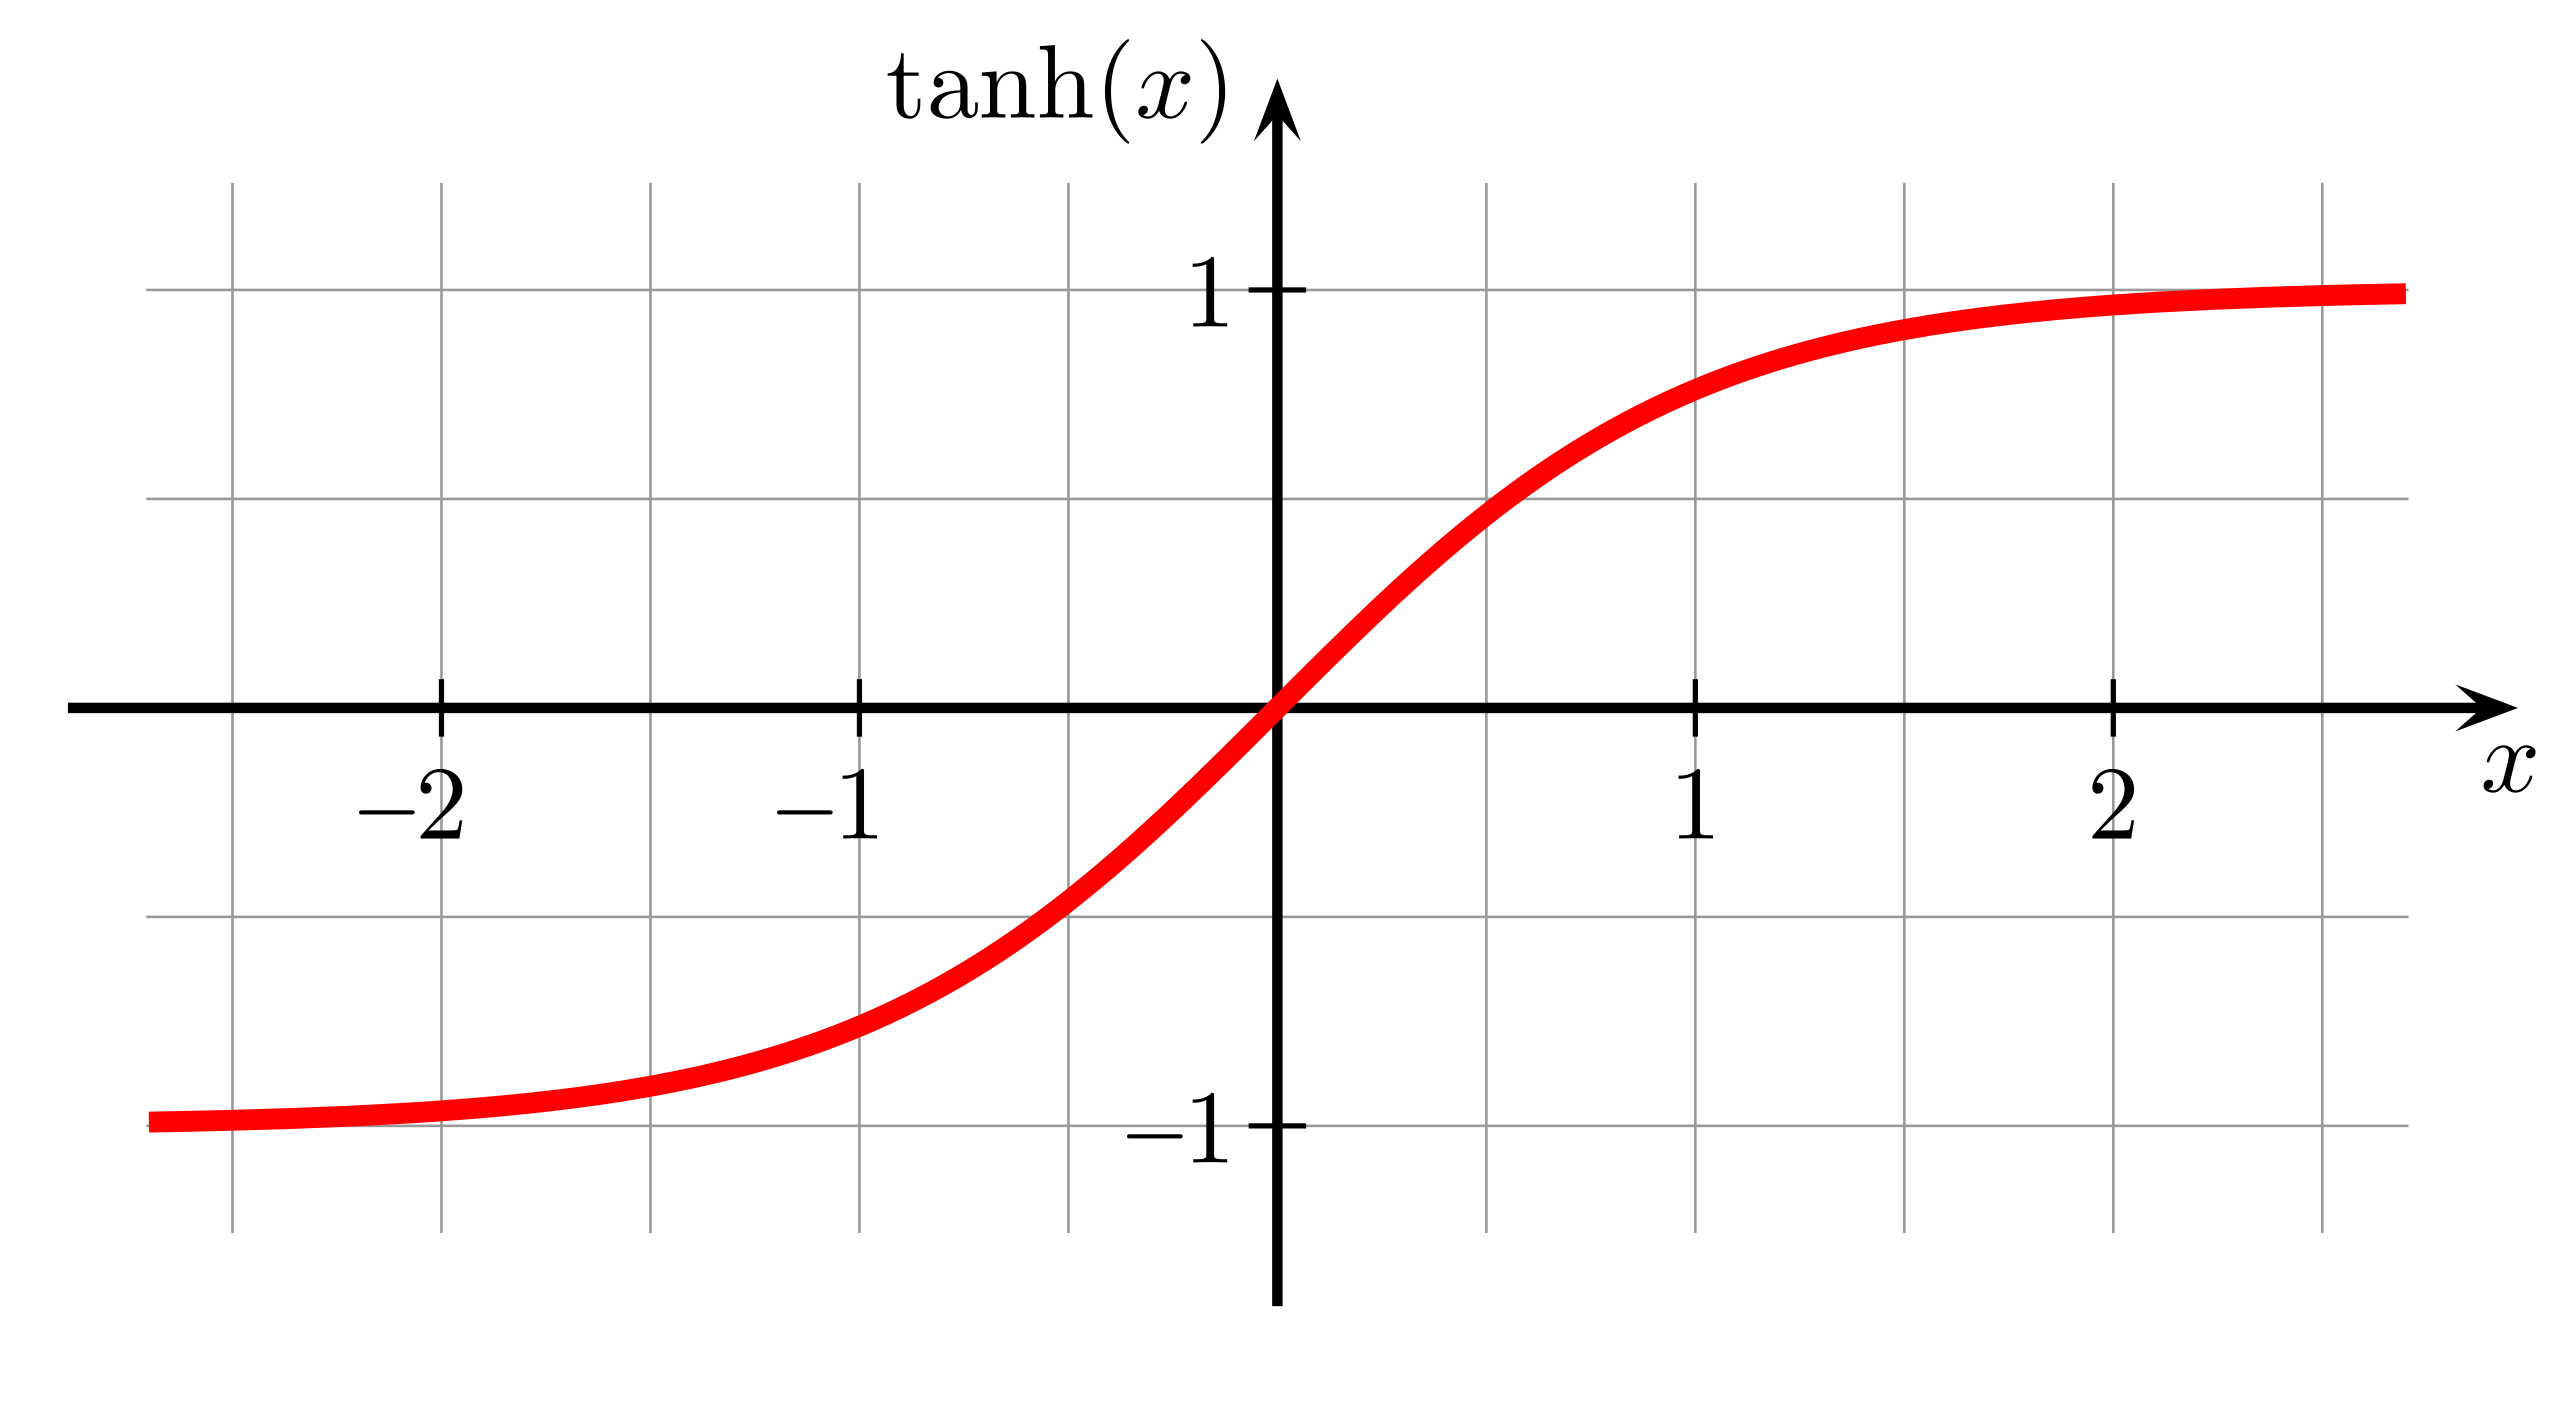
\includegraphics[width=8cm]{tanh.png}
        \end{center}
        
    \item \textbf{ReLU: }$g(z) = \max(0,z)=a$\\
    \begin{equation*}
        a' =
          \begin{cases}
            1 & \text{for x $>$ 0}\\
            0 & \text{for x $<$ 0}
          \end{cases}       
      \end{equation*}
    \\ReLU stands for Rectified Linear Unit. It is used universally, as it is considered to be better than tanh and sigmoid. This because as large $z$ values, the gradient of sigmoid and tan h functions become almost zero. Hence, gradient descent takes a lot of time to converge. ReLU does not have this problem, as the gradient is 1 for $z>0$.
        \begin{center}
            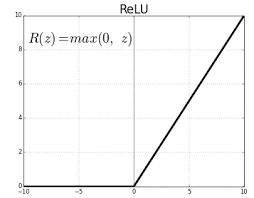
\includegraphics[width=8cm]{relu2.png}
        \end{center} 
    \item \textbf{Leaky ReLU: }$g(z) = \max(\alpha z,z)$\\
    \begin{equation*}
    a' =
      \begin{cases}
        1 & \text{for x $>$ 0}\\
        \alpha & \text{for x $<$ 0}
      \end{cases}       
  \end{equation*}   
    \\Leaky ReLU is a slight variation of the ReLU function, where the function is not zero for $z<0$, but a value $\alpha z$, where $\alpha$ is a small positive number. This helps solve the Dying ReLU problem, where a neuron with a negative bias would never activate, as the gradient would be zero.
        \begin{center}
            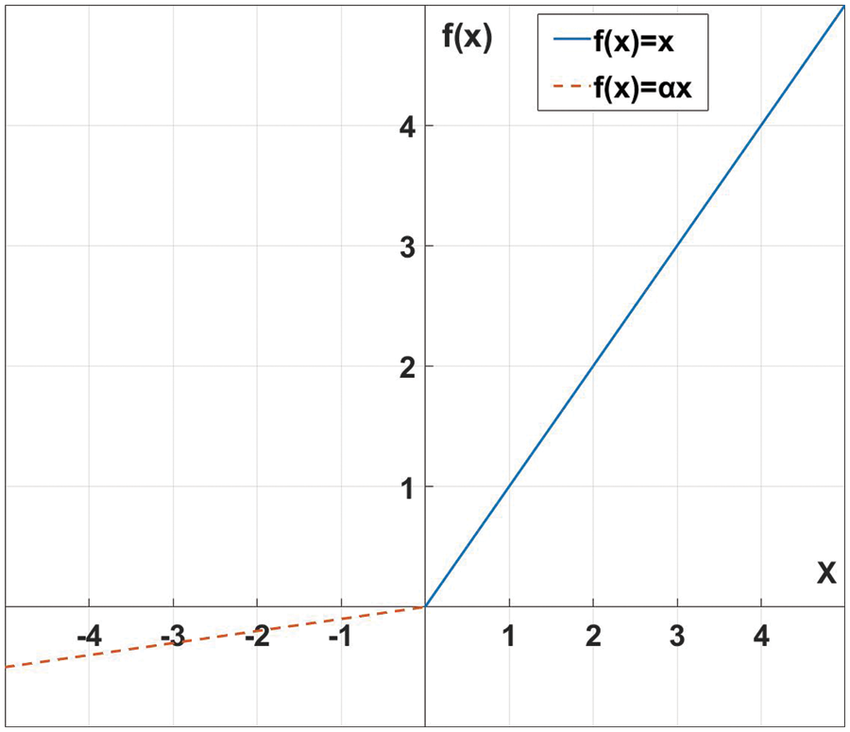
\includegraphics[width=8cm]{leaky-relu.png}
        \end{center}
\end{itemize}





\newpage
\section{Updated POA}
\begin{itemize}
    \item \textbf{Week 1: }Got familiar with various python libraries like numpy, matplotlib and pandas
    \item \textbf{Week 2: }Got started with Andrew Ng's course on Supervised Machine Learning: Regression and Classification
    \item \textbf{Week 3: }Completed the course and got an overview of the mathematics behind linear, polynomial and logistic regression from Trevor Hastie
    \item \textbf{Week 4: }Read about classification algorithms like Naive Bayes and SVMs from JakeVandeplas, Trevor Hastie and Deisenroth, and completed the midterm report submission
    \item \textbf{Week 5: }Get started with the Advanced Learning Algorithms course by Andrew Ng and read about the remaining learning algorithms like Random Forests, K-Means, from JakeVandeplas.
    \item \textbf{Week 6: }Delve into deep learning and Read about RNN’s and CNN’s from Eli Stevens and Andrew Ng’s course on Deep Learning
    \item \textbf{Week 7: }Check/Try out implementations of these deep learning models
    \item \textbf{Week 8: }Go over some of the mathematics behind these ML algorithms from Deisenroth and complete the final report submission. Also read about special concepts like Recommender Systems, Anomaly detection and bias-variance tradeoff.
\end{itemize}
\newpage
\begin{thebibliography}{9}

\bibitem{book1}An introduction to Statistical Learning, Hastie et al.
\bibitem{book2}Mathematics for Machine Learning, Deinsenroth et al.
\bibitem{nb1}Python Data Science Handbook, Jake VanderPlas \url{https://jakevdp.github.io/PythonDataScienceHandbook/}
\bibitem{course1} Supervised Machine Learning: Regression and Classification, Andrew Ng \url{https://www.coursera.org/specializations/machine-learning-introduction}
\bibitem{yt1}Statquest with Josh Starmer: \url{https://www.youtube.com/@statquest}
\bibitem{book3}Understanding Machine Learning: From Theory to Algorithms, Shai Shalev-Shwartz and Shai Ben-David

\end{thebibliography}

\end{document}

